\hyt{ladovskazima}
\song{Ladovská zima}
\note{capo 5}
\vspace{15pt}

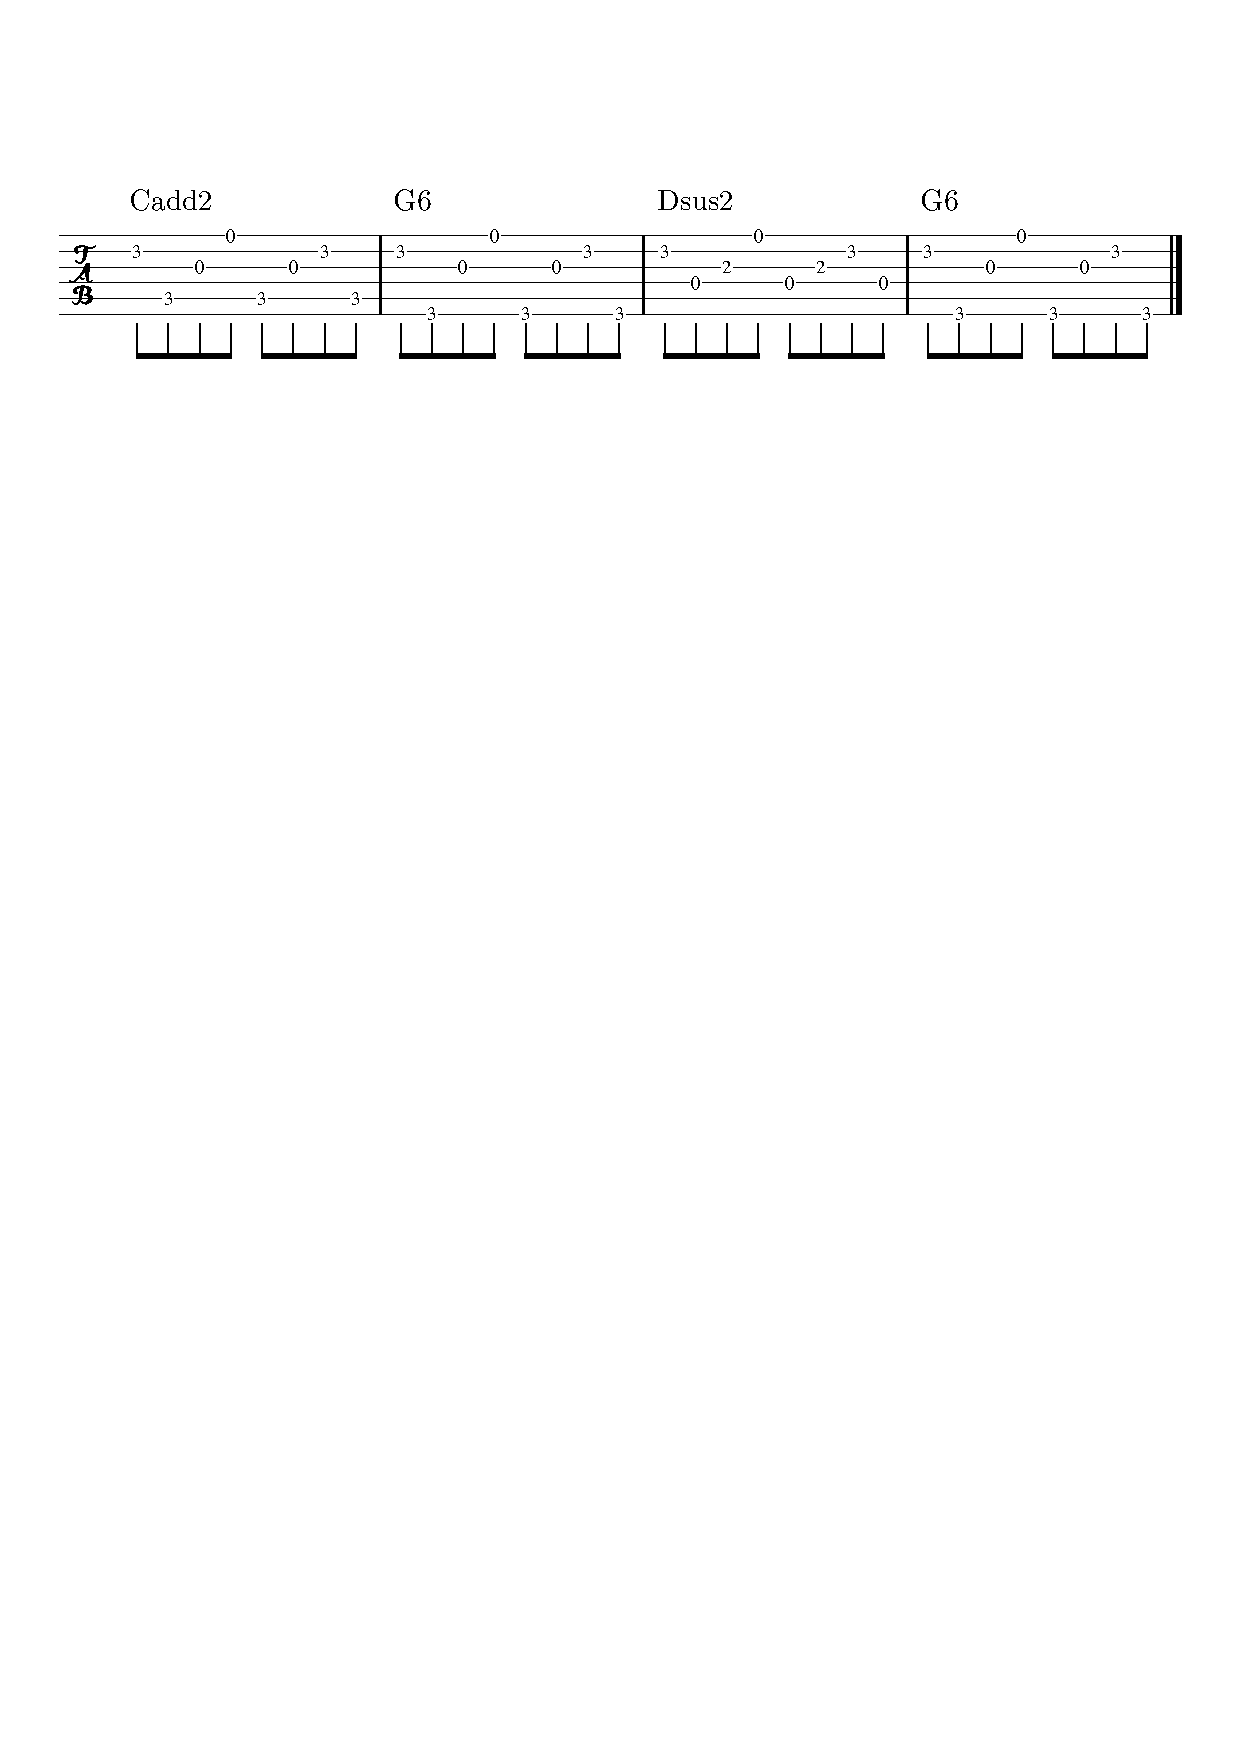
\includegraphics[width=\linewidth]{scores/ladovskazima.pdf}

\vers{1}{
Za vločkou vločka z oblohy padá, chvilinku počká, a potom taje.\\
Na staré sesli sedí pan Lada, obrázky kreslí zimního kraje.
}

\refrain{
Ladovská zima za okny je a srdce jímá bílá nostalgie.\\
Ladovská zima, děti a sáně a já jdu s nima do chrámu Páně.\\
Bim bam bim bam bim bam bim bam bim bam bim.
}
\vspace{5mm}

\emph{rec:} To mokre bile svinstvo pada mi za limec, už štvrty měsic v jednym kuse furt prosinec.\\
Večer to odhažu, namažu zada, rano se vzbudim a zas kurva pada.
\vspace{2mm}

\nv Děcka maju zmrzle kosti, saňkuju už jenom z povinnosti.\\
Mrzne jak sviňa, třicet pod nulu, auto ani neškytne, hrudky se dělaji v Mogulu.
\vspace{2mm}

\nv Kolony aut krok-sun-krok, bo silničaři, tak jak každy rok,\\
su překvapeni velice, že snih zasypal jim silnice.
\vspace{2mm}

\nv Pendolino stoji kdesik u Polomi, zamrzly mu všecky CD-ROMy.\\
A policajti? Ti to jisti z dalky - zalezli do Aralky. \refsm{}
\vspace{5mm}

\nv Na Vysočině zavřeli D jedničku, kamiony hraly na honičku.\\
Takzvane \uv{Rallye letni gumy} v tym kopcu u Meziřiči,\\
spěchaly s melounama a teď jsou v\dots však vite kde.
\vspace{2mm}

\nv Na ČT1 studio Snih, Voldanova sedi na sanich.\\
A v Praze kalamita jak na Sibiři: tři centimetry sněhu! A u Muzea čtyři.
\vspace{2mm}

\nv Jak v dalce vidim zasněženy Řip, řikam si,\\
praotče Čechu, tys byl ale strašny cyp.\\
Kdyby si popošel eště o par kilometru dale,\\
tak sem se teďka mohl kdesi v teple v plavkach valet.
\vspace{2mm}

\nv A misto toho, aby se člověk bal zajit do Tesca na nakupy,\\
jak sou na tych rovnych střechach sněhu kupy.\\
Do toho všeho, jak mam zmrzly nos aj lica,\\
tak eště z radia provokater Nohavica. \refsm{}
\newpage
